\subsection{Timing Performance Results for Laser Pulses}
\label{sec:lasertiming}

To evaluate the impact of the intrinsic timing performance of the SiPMs
on the time resolution measured for the sampling calorimeter signals, 
we performed laser-based measurements for two types of SiPMs: a Hamamatsu
S12571-015P Multi-Pixel Photon Counter (MPPC) with an area of $1\times
1$~$\mathrm{mm}^{2}$ and pixel pitch size of $15$~$\mu$m, and a Hamamatsu
S12572-25C MPPC with an area of $3\times 3$~$\mathrm{mm}^{2}$ and pixel pitch
size of $25$~$\mu$m. Examples of the digitized waveforms for signals from both
SiPMs are shown in Figure~\ref{fig:pulses}.

\begin{figure}[htbp] 
\centering
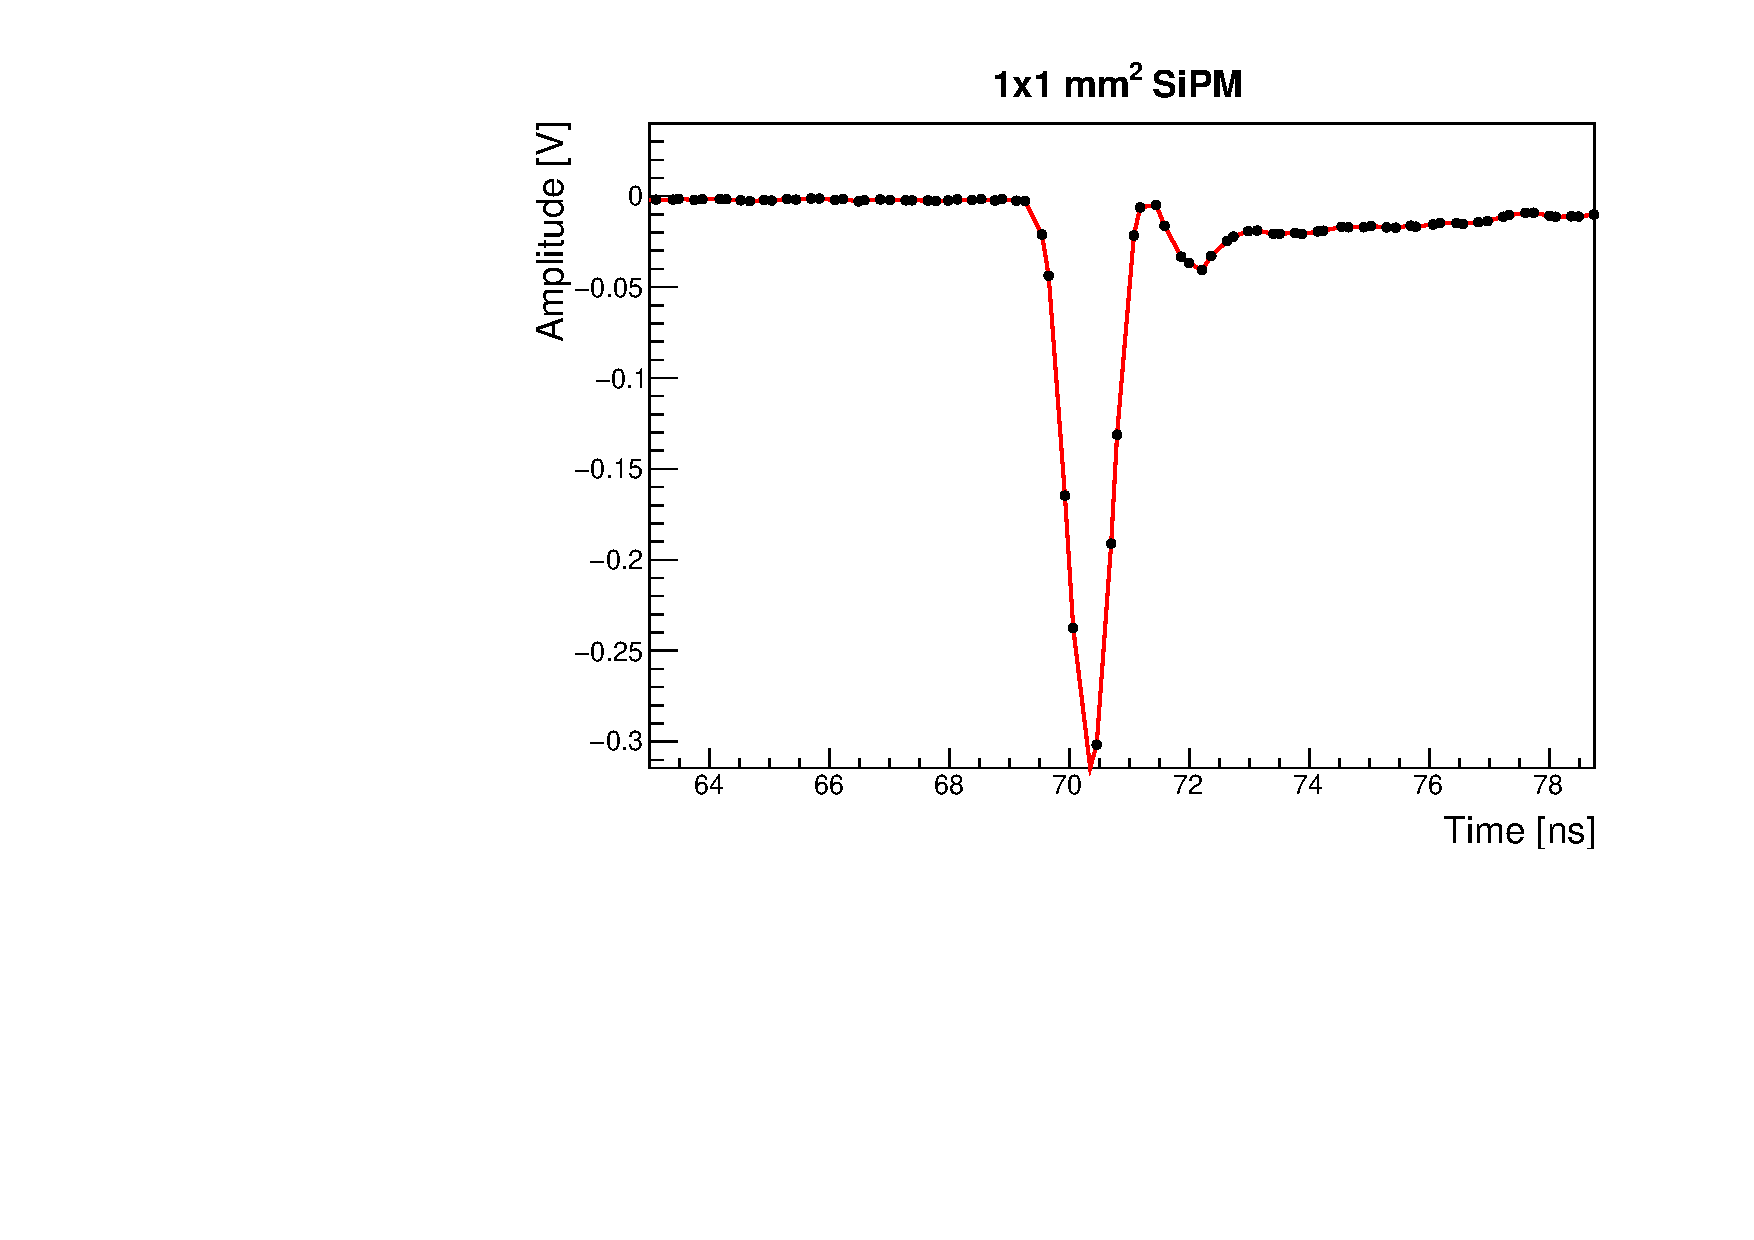
\includegraphics[width=0.49\textwidth]{figures/PulseShapeExample_1x1SiPM.pdf} 
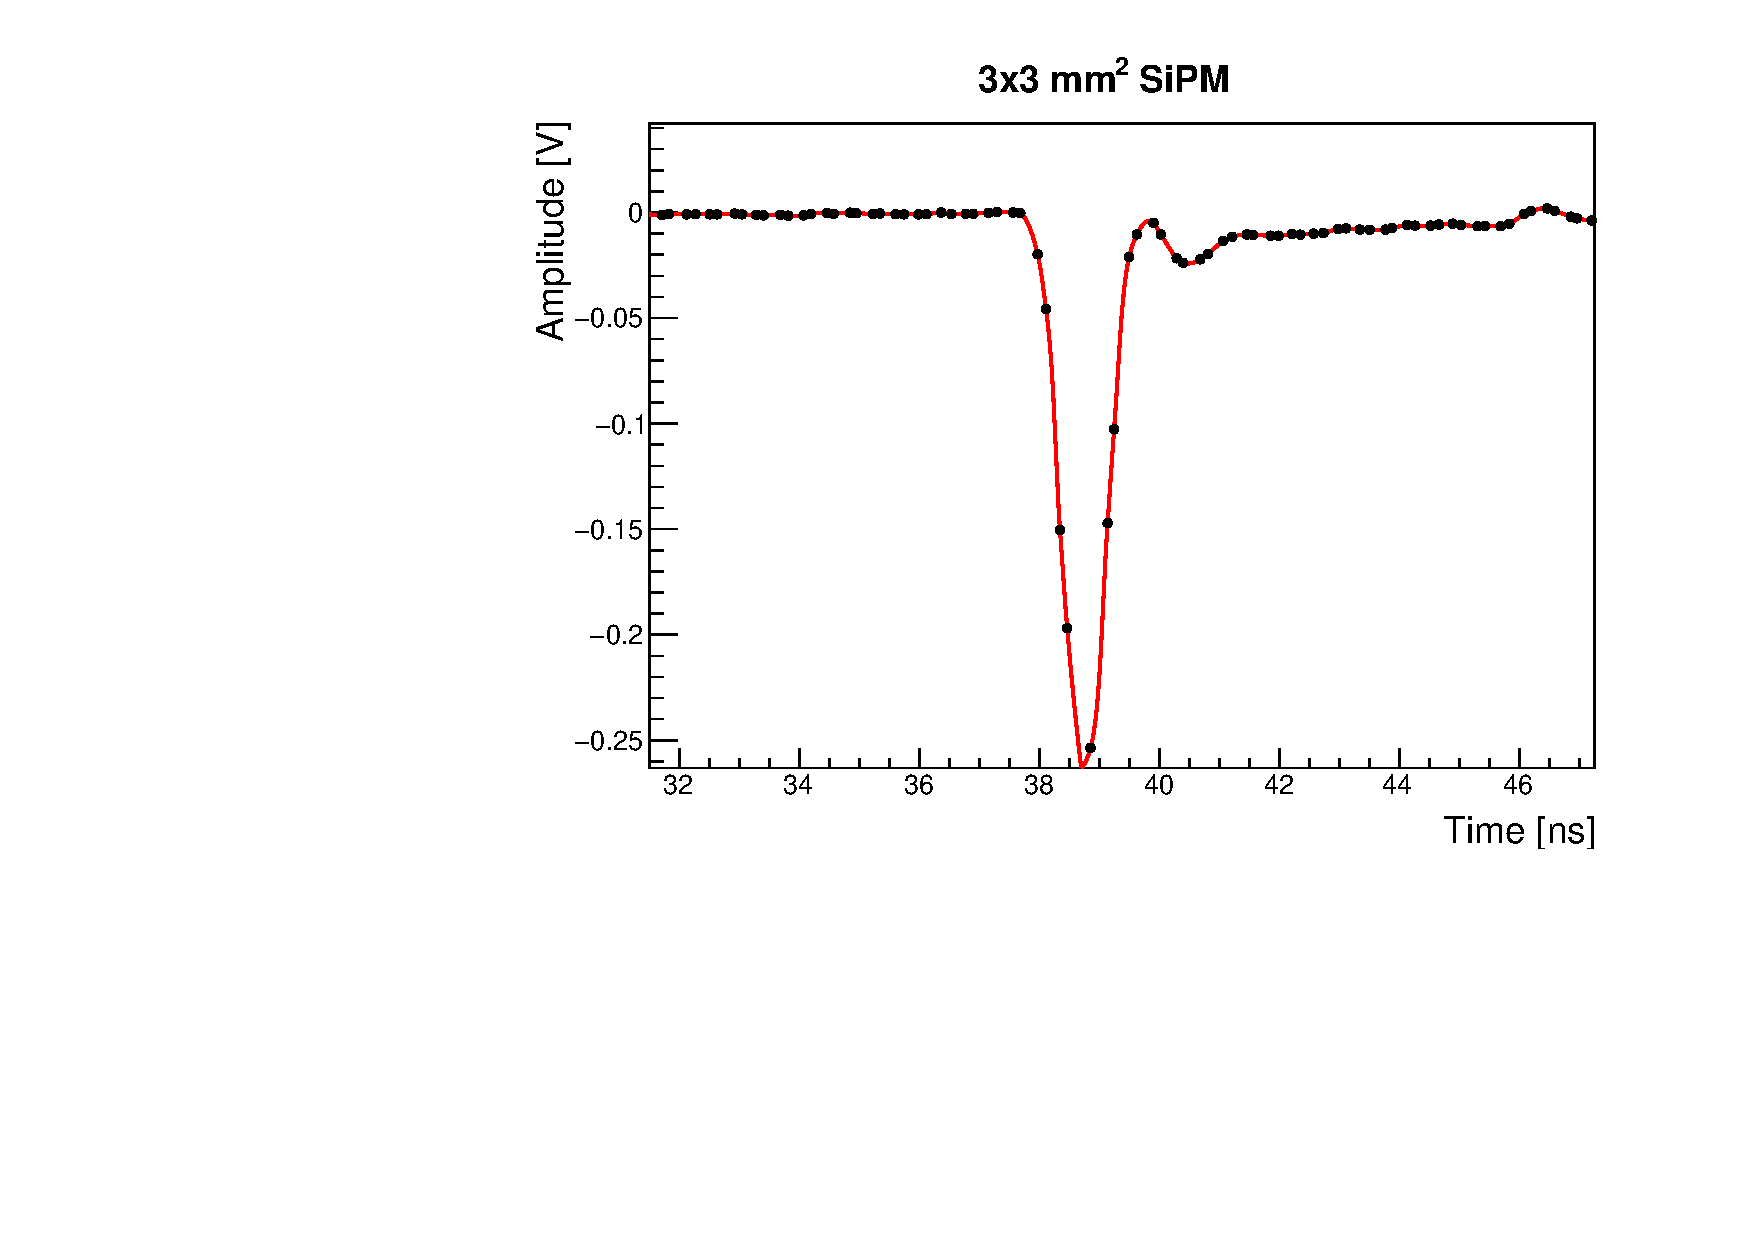
\includegraphics[width=0.49\textwidth]{figures/PulseShapeExample_3x3SiPM.pdf} 
\caption{Digitized waveforms of the signals from the PiLas laser 
in the S12571-015P and S12572-25C SiPMs.} 
\label{fig:pulses} 
\end{figure} 

Using several different ND filters we controlled the intensity of the photon 
beam impinging upon the SiPMs under test and achieved a large dynamic range 
of signal sizes ranging from a single incident photon to a few hundred. In 
Figure~\ref{fig:NPhotonPeaks}, we show the integrated charge distribution
for two example scenarios from which we can clearly distinguish different peaks
corresponding to different number of photoelectrons detected by the SiPMs.

\begin{figure}[htbp] 
\centering
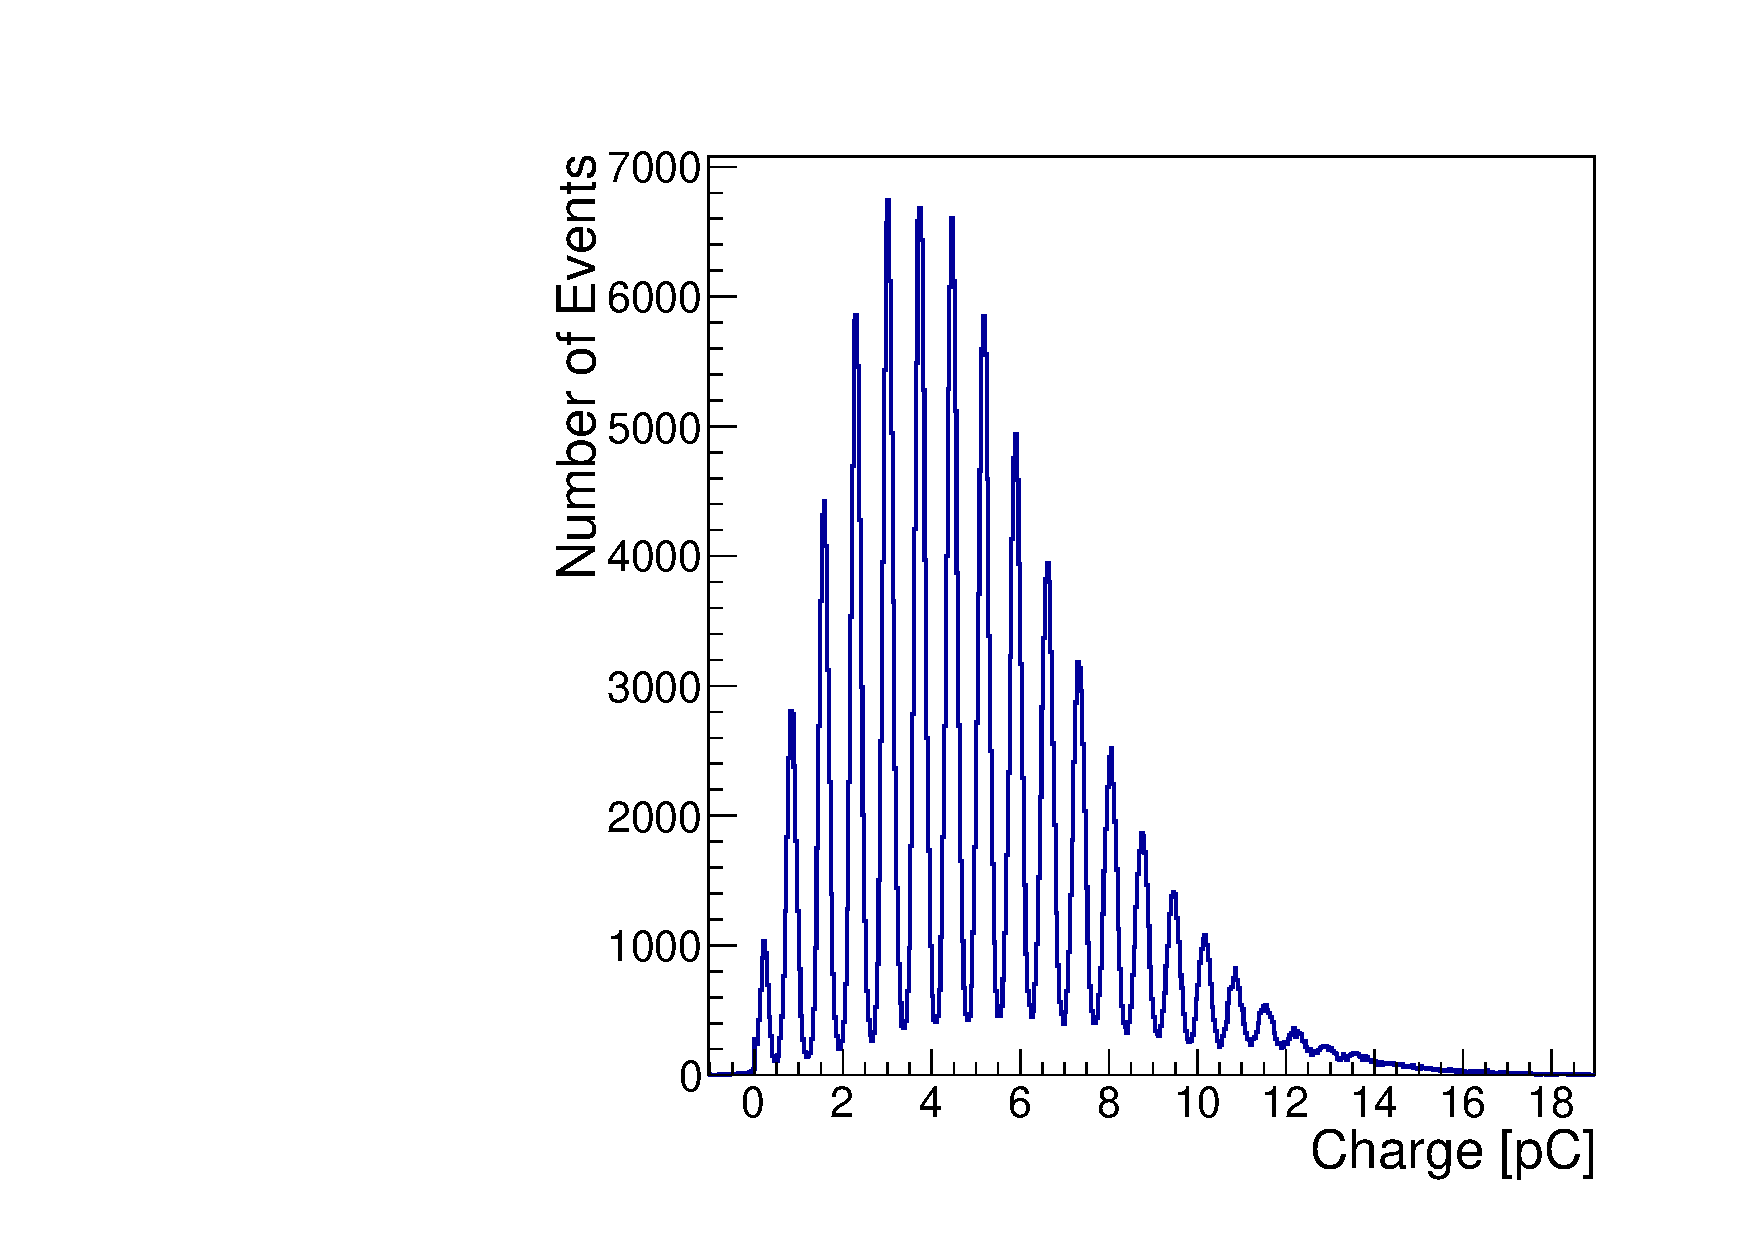
\includegraphics[width=0.49\textwidth]{figures/NPhotons1.pdf} 
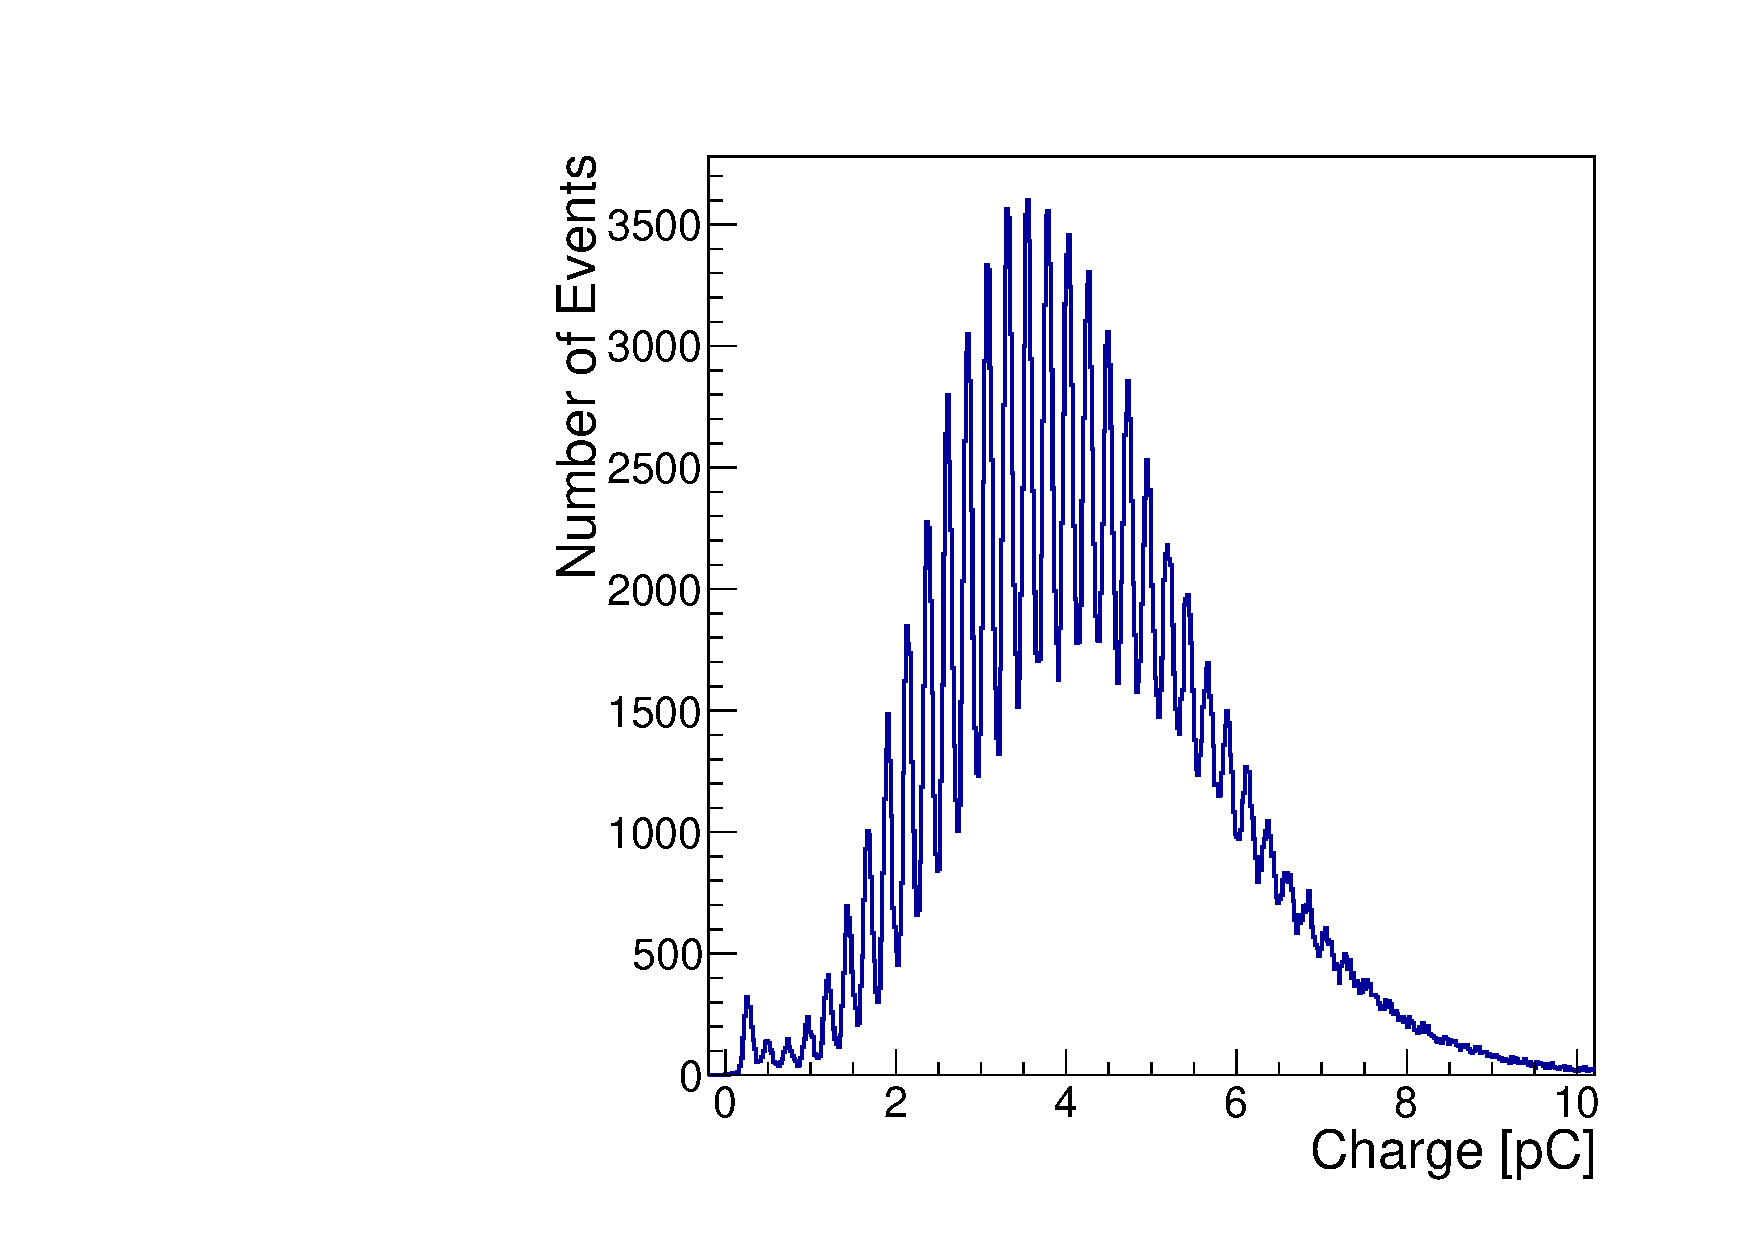
\includegraphics[width=0.49\textwidth]{figures/NPhotons2.pdf} 
\caption{The distribution of integrated charge from the SiPM sensor for data 
taken with an ND filter of 1.8 (left), and an ND filter of 1.4 (right). 
A $10$~db attenuator has been used for the plot on the right. The peaks corresponding
to different discrete numbers of photoelectrons detected by the SiPM is clearly
evident.} 
\label{fig:NPhotonPeaks} 
\end{figure} 

Using this setup, we measure the timestamps reconstructed from the SiPM signals
with respect to the reference MCP-PMT timestamp over an ensemble of events
triggered by the external laser trigger. The sigma parameter of a gaussian fit
to this distribution is taken as the time resolution measurement.
As the number of photons impinging on the SiPM can be clearly distinguished 
based on the amplitude or charge collected, we can study the dependence of the 
time resolution on the number of photons. These measurements are shown in 
Figure~\ref{fig:TimeResolutionVsNPhotons}. The amplitude for a single
photoelectron signal is estimated to be $0.6$~mV for the $1\times1$~$\mathrm{mm}^{2}$ 
S12571-015P SiPM and $0.1$~mV for 
the $3\times 3$~$\mathrm{mm}^{2}$ S12572-25C SiPM. Using these 
measurements, we can compare the time resolution of laser light signals on
SiPMs from Figure~\ref{fig:TimeResolutionVsNPhotons} to the time resolution
of electromagnetic shower signals from the WLS fiber in Figure~\ref{TimeResolution}
and conclude that the impact of the intrinsic timing performance of 
SiPM devices are small and between a factor of $8$ and $10$ smaller. 
Therefore the time resolution of the calorimeter is dominated by the 
impact of the wavelength shifter and the increased rise time.
An additional contribution to the timing resolution of the calorimeter cell may
arise from longitudinal shower fluctuations. Shower depth fluctuations result in
fluctuations in the time it takes for the shower to propagate into the
calorimeter cell as well as for the scintillation light to propagate out of the
cell thought the light guides. This contribution of the shower fluctuations only
manifest themselves if the signal is extracted on the front of the calorimeter
cell, where a depth fluctuations is not compensated by a corresponding reduction
in the optical signal transport path length. Such effects have been observed in
timing studies for the CMS ECAL \cite{ecaltimingconfnote}.

\begin{figure}[htbp] 
\centering
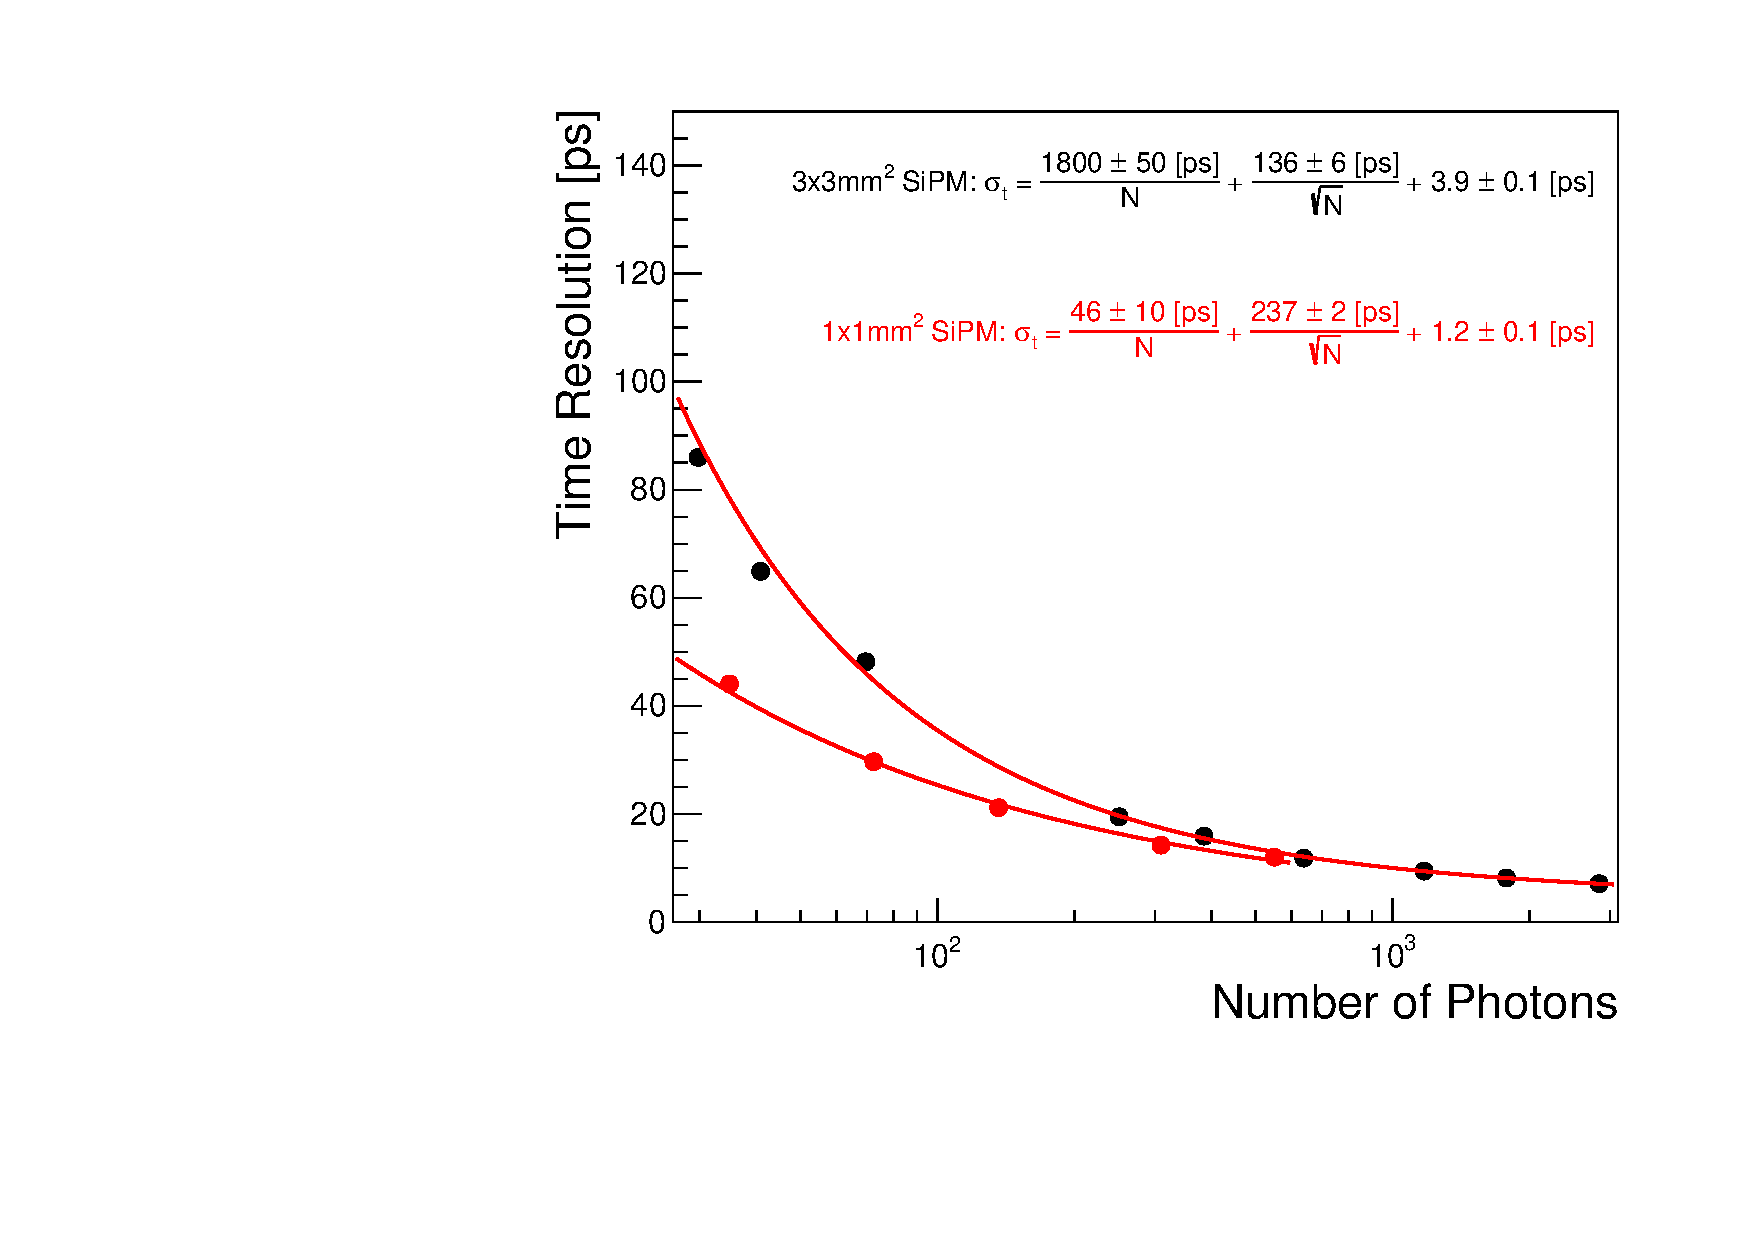
\includegraphics[width=0.8\textwidth]{figures/TimeResolutionVsNPhotons.pdf}
\caption{ The time resolution is measured as a function of the number of photons 
impinging on the SiPMs under test. The black points show measurements using the
$3\times3$~$\mathrm{mm}^{2}$ SiPM, and the red points show measurements
using the $1\times1$~$\mathrm{mm}^{2}$ SiPM. \label{fig:TimeResolutionVsNPhotons}
} 
\end{figure} 


Finally, by removing all ND filters and increasing the laser output intensity to near 
maximum, we can measure the time resolution for a very large number of photons 
to probe for the ultimate time resolution that one could achieve with a near 
infinitely large signal. In Figure~\ref{fig:LargeLightTimeResolution} we show 
the SiPM time distributions for such a scenario, and observe that the resolution 
is $12$~ps for the $1\times1$~$\mathrm{mm}^{2}$  S12571-015P SiPM and
$7$~ps for the $3\times 3$~$\mathrm{mm}^{2}$ S12572-25C SiPM. 
The measurement is also impacted by the limitation
of the digitizer electronics as its impact on the time resolution is $4$~ps. 

\begin{figure}[htbp] 
\centering
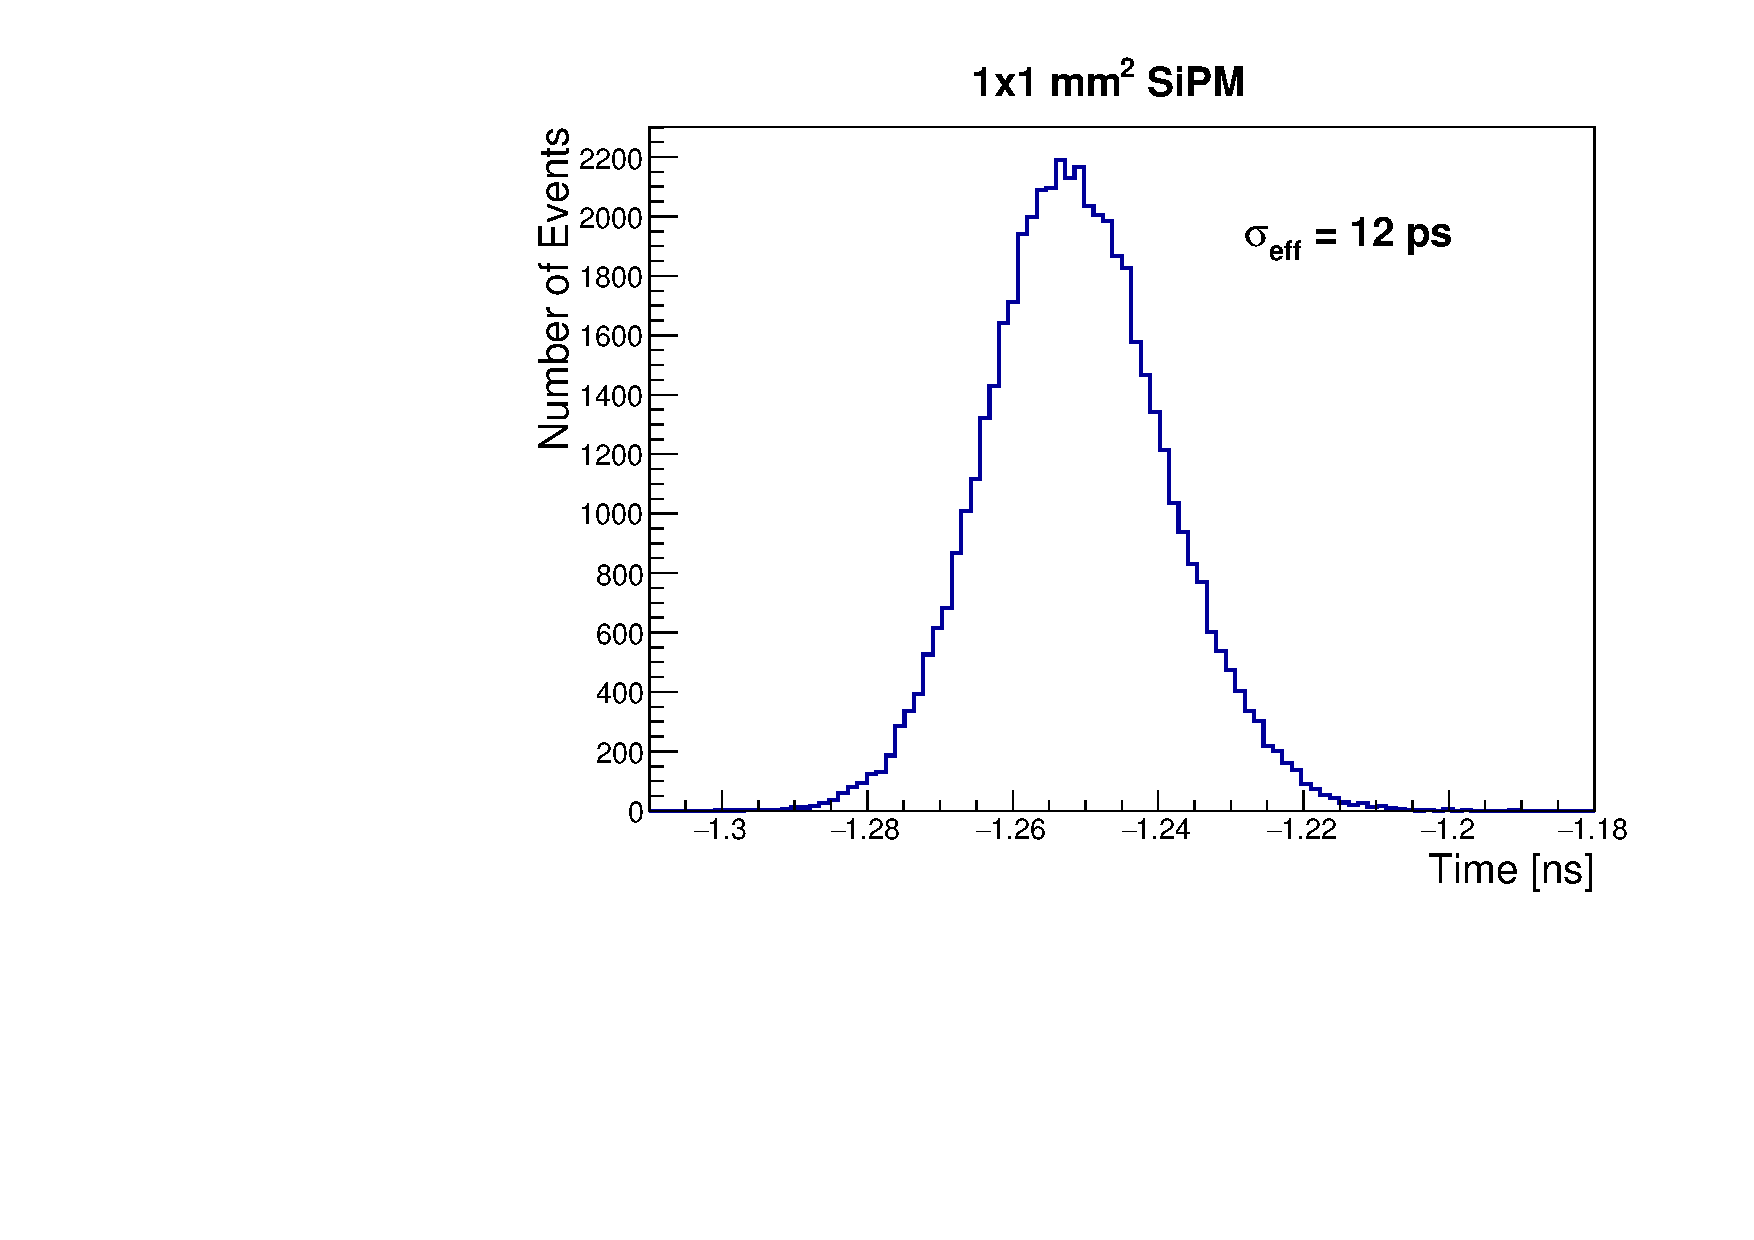
\includegraphics[width=0.49\textwidth]{figures/DeltaT_LargeNPhotons_1x1SiPM.pdf} 
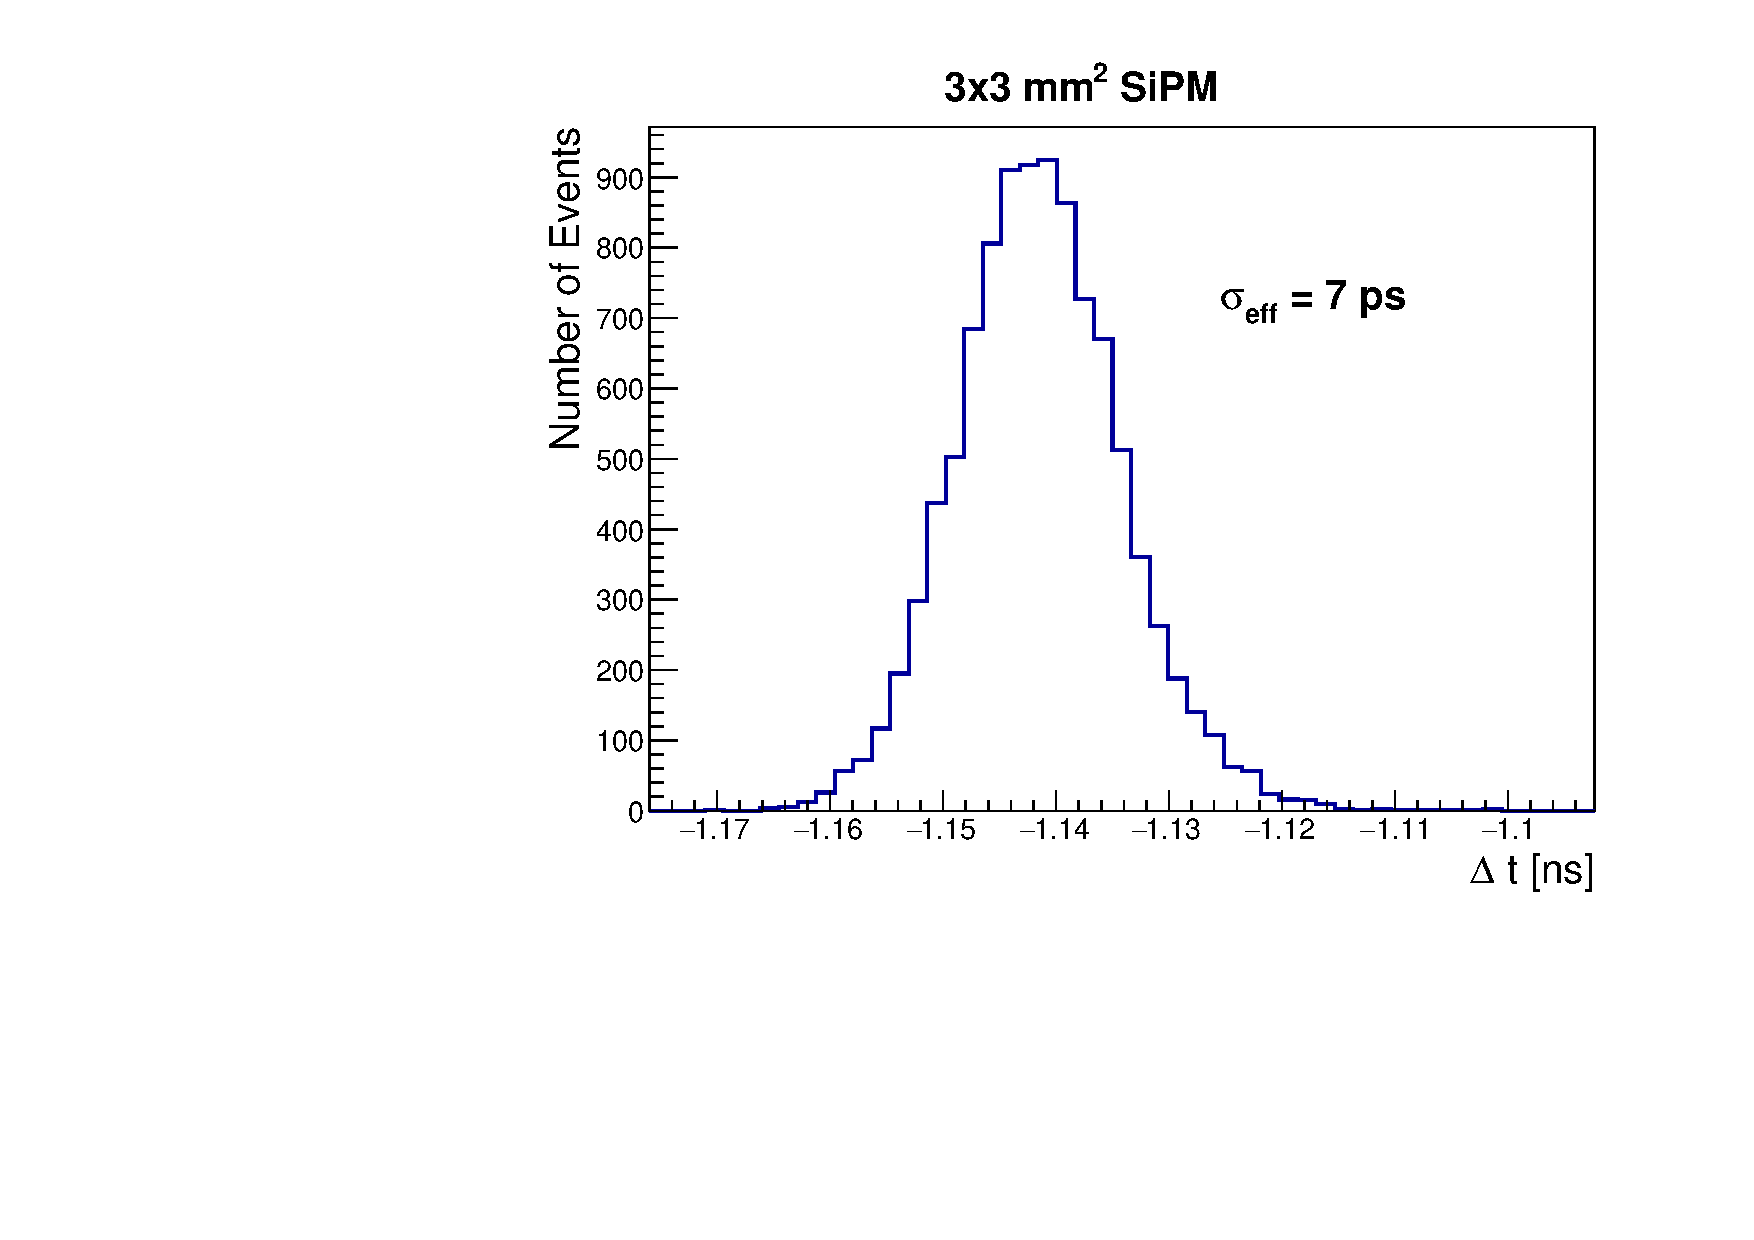
\includegraphics[width=0.49\textwidth]{figures/DeltaT_LargeNPhotons_3x3SiPM.pdf} 
\caption{The SiPM time distribution and resolution measured for laser signals at high laser intensity.} 
\label{fig:LargeLightTimeResolution} 
\end{figure} 

